%%%%%%%%%%%%%%%%%%%%%%%%%%%%%%%%%%%%%%%%%
% LaTeX Template
% http://www.LaTeXTemplates.com
%
% Original author:
% Linux and Unix Users Group at Virginia Tech Wiki 
% (https://vtluug.org/wiki/Example_LaTeX_chem_lab_report)
%
% License:
% CC BY-NC-SA 3.0 (http://creativecommons.org/licenses/by-nc-sa/3.0/)
%
%%%%%%%%%%%%%%%%%%%%%%%%%%%%%%%%%%%%%%%%%

%----------------------------------------------------------------------------------------
%	PACKAGES AND DOCUMENT CONFIGURATIONS
%----------------------------------------------------------------------------------------

\documentclass[12pt]{article}
\usepackage{geometry} % Pour passer au format A4
\geometry{hmargin=1cm, vmargin=1cm} % 

\usepackage{graphicx} % Required for including pictures
\usepackage{float} % 

%Français
\usepackage[T1]{fontenc} 
\usepackage[english,francais]{babel}
\usepackage[utf8]{inputenc}
\usepackage{eurosym}
\usepackage{lmodern}
\usepackage{url}
\usepackage{multicol}
\usepackage{multido}

%Maths
\usepackage{amsmath,amsfonts,amssymb,amsthm}
%\usepackage[linesnumbered, ruled, vlined]{algorithm2e}
%\SetAlFnt{\small\sffamily}

%Autres
\linespread{1} % Line spacing
\setlength\parindent{0pt} % Removes all indentation from paragraphs

\newcommand{\horrule}[1]{\rule{\linewidth}{#1}} % Create horizontal rule 
\renewcommand{\labelenumi}{\alph{enumi}.} % 

\newcommand{\Pointille}[1][3]{\multido{}{#1}{    \makebox[\linewidth]{\dotfill}\\[\parskip]}}

\pagestyle{empty}
%----------------------------------------------------------------------------------------
%	DOCUMENT INFORMATION
%----------------------------------------------------------------------------------------
\begin{document}
\setlength{\columnseprule}{1pt}

%\maketitle % Insert the title, author and date

\textbf{Nom(s), Prénom(s) :}

\begin{center}
  \textit{La normalité est une route pavée : on y marche aisément mais les fleurs n'y poussent pas.}\\ \textbf{- Vincent Van Gogh -}
\end{center}

\textbf{Pour toutes les questions, il est demandé de laisser apparaître une trace des calculs et de répondre à la question par une phrase.}


\textbf{Exercice 1}

\begin{multicols}{2}

  \begin{enumerate}
  \item[a.] Dans un garage, 12 des 20 voitures sont des voitures ``diesel''. Calculer le pourcentage de voitures ``diesel'' dans ce garage.\\
    \Pointille[5]
  \item Sur 150 paires de ski fabriquées, 19 avaient un défaut. Calculer le pourcentage de paires de skis qui avaient un défaut.\\
    \Pointille[5]
  \end{enumerate}

\end{multicols}


\begin{multicols}{2}

  \textbf{Exercice 2}\\
  Lors d'un tournoi de pétanque, Marius a réussi 37 tirs sur 48 alors que Chloé en a réussi 31 sur 40. Lequel de ces deux joueurs a eu le pourcentage de réussite le plus élevé ?\\ \vspace{0.5cm}
  \Pointille[7]

\end{multicols}

\textbf{Exercice 3}\\
Avec la calculatrice, calculer la masse d'eau contenue dans chacun de ses fruits.

\begin{multicols}{2}
  \begin{enumerate}
  \item[a.] 
    \begin{figure}[H]
      \centering
      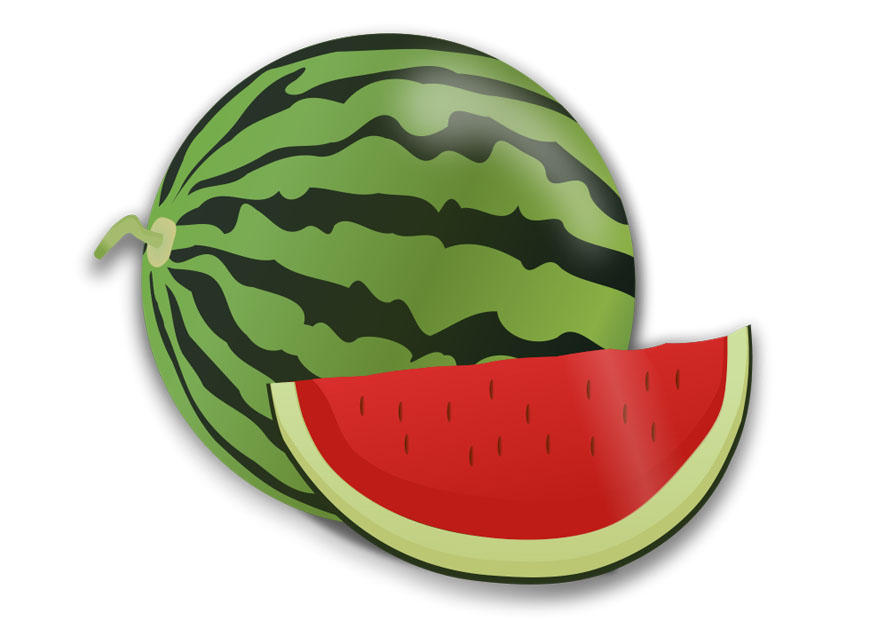
\includegraphics[width=0.3\linewidth]{sources/2/pasteque.jpg}
    \end{figure}
    Pastèque\\
    Masse : 540g\\
    Eau : 95\%\\
    \Pointille[3]

  \item [b.]
    \begin{figure}[H]
      \centering
      
\includegraphics[width=0.2\linewidth]{sources/2/pomme.jpg}
    \end{figure}
    Pomme\\
    Masse : 185g\\
    Eau : 84\%\\
    \Pointille[3]
  \end{enumerate}
\end{multicols}


\begin{multicols}{2}
  \textbf{Exercice 4}\\
  Entre 1900 et 2010 les tailles moyennes des Français (femmes : $1,54m$ ; hommes : $1,66m$) ont augmenté d'environ $6,5\%$. Calculer les tailles moyennes en m des femmes et des hommes en 2010 (on donnera les valeurs approchées par défaut au centième près).\\

  \Pointille[6]

\end{multicols}

\end{document}
